\documentclass[letterpaper]{article}
\usepackage[pdftex]{graphicx}
\usepackage{tp}
\usepackage{unitsdef}
\usepackage{pifont}
\usepackage{sectsty}
\usepackage{amsmath}
\usepackage{eso-pic}
\usepackage[T1]{fontenc}
\usepackage{varioref}
\usepackage{caption}
\usepackage{textcomp}
\usepackage{float}
\usepackage{epsfig}
\usepackage{tikz}
\usetikzlibrary{arrows}
\pagestyle{plain}
\renewcommand{\arraystretch}{1.4}
\begin{document}
\usefont{T1}{ua1}{m}{n}\selectfont
\newcommand{\tfont}{\usefont{T1}{ua1}{m}{n}\selectfont\footnotesize}
\newcommand{\bfont}{\usefont{T1}{ua1}{b}{n}\selectfont\tiny}
\newcommand{\xfont}{\usefont{T1}{ua1}{m}{n}\selectfont\scriptsize}
\newcommand{\lfont}{\usefont{T1}{ua1}{m}{n}\selectfont\large}
\renewcommand{\captionfont}{\it }
\renewcommand{\date}{February 26, 2020}
\newcommand{\ver}{V1.0}
\newcommand{\tablecap}{\hline\end{tabular}\end{table}\end{center}}
\renewcommand{\versionhistory}{
\vspace*{1in}
\begin{center}
\begin{table}[H]\caption*{Revision History}
\centering
\xfont\begin{tabular}[H]{|c|c|c|c|}
\hline
{\bf Version} & {\bf Author} & {\bf Date} & {\bf Changes}\\
\hline
\hline
1.0 & Eric West & 2/26/20 & Initial Release \\
\hline
\end{tabular}
\end{table}
\end{center}
}
\maketitle
\setcounter{tocdepth}{3}
\tableofcontents
\clearpage
\makebg

\section{\bf Introduction}
stdf2xls 5.0 is a program that converts STDF files into spreadsheets, wafermaps, and/or histograms.
It is natively compiled from the D-language and therefore it uses much less memory than the previous
stdf2xls 4.0 java program, and is significantly faster too.  It has many new features:
\begin{itemize}
\item Spreadsheet and ASCII wafermaps
\item Spreadsheet histograms
\item Ability to display hex, integer, and string data values in the spreadsheet
\item New algorithm correctly orders tests even if the testflow varies from device to device
\item Spreadsheet colors and fonts are now customizable
\item Improved spreadsheet layout
\item Many ways to sort and order device data, including by timestamp
\item Ability to modify any STDF text field with regular expressions
\item Ability to write out STDF files
\item Multiple different devices types can be processed simultaneously
\end{itemize}

There are a couple of minor regressions though:
\begin{itemize}
\item No more support for big-endian CPUs.
It seems that most testers today are using the Intel CPU architecture,
so why pay for the performance penalty if you don't need it.
\item Logo scaling is more difficult.  This is because of
the new xlsx library being used which makes image handling
a little more difficult.
\end{itemize}

\section{\bf Getting the program}

The source code is available on github. The source code can be downloaded
from github with git, or just the executable for Windows or GNU/Linux
may be downloaded from the github web page.  This manual may also be copied
from the github webpage.\\
\\
To download the software with git use the following command:
\begin{verbatim}
git clone https://github.com/itestinc/stdf2xls.git
\end{verbatim}

\noindent To compile the source code on GNU/Linux you also need dub, gcc and dmd (dmd is the D compiler).

\section{\bf Installation}

To just install the executable, the program can be downloaded from github.com.

\subsection{\bf GNU/Linux Installation}

For GNU/Linux go to https://github.com/itestinc/stdf2xls, click on the dist folder, then
click on the stdf2xls file, then press the Download button.  After the file has downloaded
put it in a directory that in in your executable search path.

\subsection{\bf Windows Installation}

First, you must have the Windows SDK installed on your computer.  It can be obtained at:\\
https://developer.microsoft.com/en-us/windows/downloads/windows-10-sdk The program will also work on Windows7.\\
\\
\noindent
For Windows go to https://github.com/itestinc/stdf2xls, click on the dist folder, then 
click on the stdf2xls.exe file, then press the Download button.  After the file has downloaded
put it in a directory that in in your executable search path.

\section{\bf Usage}

A summary of the command line options can be printed by running the program
with the '\texttt{-{}-}help' option.  More detailed information about the command line
options is given in this manual.
\begin{verbatim}
stdf2xls --help or stdf2xls -h
\end{verbatim}
gives the following output:
\begingroup
\scriptsize
\begin{verbatim}
Options:
-a        --extract-pin Extract pin name from test name suffix (default delimiter = '@')
-b          --dumpBytes dump the STDF in ascii byte form
-d           --dumptext dump the STDF in text form
-m             --modify modify a string field in specified record type.
Example: -m 'MIR TST\_TEMP "TEMPERATURE :" "TEMPERATURE:"'
-o          --outputDir write out the STDF to this directory. Specifying this will cause the STDF to be written back out.
-p      --pin-delimiter Delimiter character that separates pin name from test name (Default = '@')
-i --ignoreSerialMarker Ignore the serial marker and use STDF part ID instead
-D             --digest Summarize file contents
-s    --genSpreadsheets Generate spreadsheet(s)
-S                 --so Spreadsheet output filename(s); name may contain variables for device, and/or lot
Default = %device%_%lot%.xlsx
-r             --rotate Transpose spreadsheet so there is one device per column instead of one device per row
--sortType Sort devices by alphanumeric serial number, then by time. See the manual for valid sort types
-c              --1kcol limit to 1000 columns for libreoffice - default is 16360 columns
-Y    --noDynamicLimits Don't check for and show dynamic limits
-w       --genWafermaps Generate wafer map(s)
-W                 --wo Wafermap output filename(s); name may contain variables for device, wafer, and/or lot
Default = %device%_%lot%_%wafer%.xlsx
-A          --dumpAscii dump the wafer map in ASCII form
-f            --wformat Specify the wafermap format for the ASCII dump (default:ASY)
-P            --pattern fill wafermap bins with patterns instead of colors
-R        --rotateWafer Rotate the wafer map clockwise in degrees: +/- 0|90|180|270
-N            --showNum Show the bin numbers on the wafer map, along with colors or patterns.
-h      --genHistograms Generate histogram(s)
-H                 --ho Histogram output filename(s); name may contain variables for device, step, lot, and/or testID
Default = %device%_histograms.pdf
--binCategory Specify if bins should be divided by SITE, LOT, TEMPerature or NONE. Default = NONE
Note: if --ho contains %lot% then dividing bins by lot does not make sense
-B         --manualBins Manually set the number of bins across all histograms. Set to 0 (zero) for automatic.
-C         --cutOutlier Define how much of the outliers to cut off, in terms of standard deviation. Set to 0 (zero) for no cutoff.
-g     --generateRCFile Generate a default ".stdf2xlsxrc" file
-t       --channel-type Channel type: AUTO, CHANNEL, PHYSICAL, or LOGICAL. Only use this if you know what you are doing.
-v            --verbose Verbosity level. Default is 1 which means print only warnings.  0 means don't print anything
-V             --verify Verify written STDF; only useful if --outputDir is specified. For testing purposes only.
--noIgnoreMiscHeader Don't ignore custom user header items when comparing headers from different STDF files
-h               --help This help information.
\end{verbatim}
\endgroup

\noindent
There are nine primary operations that can be done with the program, and they may be
done individually or simultaneously:
\begin{itemize}
\item -s or \texttt{-{}-}genSpreadsheets will generate spreadsheets for the STDF measurement data
\item -h or \texttt{-{}-}genHistograms will generate histograms for the STDF measurement data
\item -w or \texttt{-{}-}genWafermaps will generate wafermaps for the STDF bin data
\item -d or \texttt{-{}-}dumptext will generate an ASCII dump of the STDF file(s)
\item -b or \texttt{-{}-}dumpBytes will generate an ASCII dump of all of the bytes in the STDF file(s)
\item -D or \texttt{-{}-}digest will dump each unique set of header information found in the STDF file(s)
\item -m or \texttt{-{}-}modify '<record> <field> ''<fromRegex>'' : ''<toRegex>'' ' will modify any text field in any record type 
\item -g or \texttt{-{}-}generateRCFile will generate an "rc" file in the home directory called ".stdf2xlsxrc"
              which contains all the default color, font, and logo settings.  This file, if it exists, is loaded
              on startup and used to configure the output.
\item -o or \texttt{-{}-}outputDir <folder\_name> will cause the STDF files that are read in to be written out to this folder
\end{itemize}

\noindent
Each of these major options have several more options to refine their behavior, and their usage
and options will be discussed in the following sections.

\subsection{\bf -s or \texttt{-{}-}genSpreadsheets}
Spreadsheet generation has nine options that control aspects of how the spreadsheet is generated.
You must give the -s or \texttt{-{}-}genSpreadsheet option to get a datalog spreadsheet.

\begin{itemize}
\item -a        \texttt{-{}-}extract-pin Extract pin name from test name suffix (default delimiter = '@')
\item -p      \texttt{-{}-}pin-delimiter Delimiter character that separates pin name from test name (Default = '@')
\item -i \texttt{-{}-}ignoreSerialMarker Ignore the serial marker and use STDF part ID instead
\item -S                 \texttt{-{}-}so Spreadsheet output filename(s); name may contain variables for device, and/or lot
\item -r             \texttt{-{}-}rotate Transpose spreadsheet so there is one device per column instead of one device per row
\item -c              \texttt{-{}-}1kcol limit to 1000 columns for libreoffice - default is 16360 columns
\item -Y    \texttt{-{}-}noDynamicLimits Don't check for and show dynamic limits
\item -t       \texttt{-{}-}channel-type Channel type: AUTO, CHANNEL, PHYSICAL, or LOGICAL.
\item -m             \texttt{-{}-}modify modify a string field in specified record type.
\end{itemize}

\subsubsection{\bf -a or --extract-pin}
Some testers like the Advantest 93K will append a pin name on to the end of a test name
to indicate the pin that is being tested.  By default it uses an \makeatletter '@' \makeatother
to delimit the test name from the pin name.  For example \makeatletter "myTestName@VCC". \makeatother
This option will remove the delimiter and pin name from the test name, and put the pin name
in the pin column or row of the spreadsheet.  You may use any character for the delimiter,
but \makeatletter '@' \makeatother is used by default.  See next section.

\subsubsection{\bf -p or --pinDelimiter}
This option allows you to specify the delimiter that is used to separate the test name and pin name.
It is only necessary to use this option if the delimiter is not \makeatletter '@'. \makeatother.
\clearpage

\subsubsection{\bf -i or --ignoreSerialMarker}
There are two ways to specify a serial number for a device.  If you do nothing then stdf2xls
will use the PART\_ID field in the PRR record as the serial number.  This field is set by the tester
automatically. However if you want to assign your own alpha-numeric serial numbers you can put
them into a Datalog Text Record using a special format.  To put your own serial numbers
in to the STDF, print a string to the datalogger using this format:
\begin{verbatim}
TEXT_DATA : S/N : <serial_id>
\end{verbatim}
For example,
\begin{verbatim}
TEXT_DATA : S/N : A1
\end{verbatim}
On the Advantest 93K a Datalog Text Record is generated by using the PUT\_DATALOG() function.
The stdf2xls program will prioritize the Datalog Text Record serial marker over the
PART\_ID field in the PRR record.  If you want to prioritize thie PART\_ID field over
the Datalog Text Record serial marker, then use this option.  Generally you won't want
to use this option.

\subsubsection{\bf -S or --so}
This option is used to specify the spreadsheet filename.  It is not necessary to use this option.
By default the spreadsheet filename will be <deviceName>\_<lot\_id>.xlsx.  Note that you can process
multiple device types simultaneously and each device and lot will be sent to a different spreadsheet
file.  With this option you can specify the datalog spreadsheet filename, and you can use variables
to specfiy the lot and/or device in the filename.  For example:
\begin{verbatim}
-S device_%device%_lot_%lot%.xlsx
\end{verbatim}
If your device was 8087 and your lot number was N5432S, then this would
give filename of\\ "device\_8087\_lot\_N5432S.xlsx"\\\\   Note that if the actual lot or device
number contains a '/' character, then the '/' will be replaced with a '\%' character
because you can't have slashes in a filename.  If the lot or device number contains
a space character, then the space will be replaced with a '\_' character.  This is because
spaces in filenames are evil.

\subsubsection{\bf -r or --rotate}
By default the datalog spreadsheet is generated with tests in columns and devices in rows.  This
option will transpose the spreadsheet so that devices are in columns and tests are in rows.

\subsubsection{\bf -c or --1kcol}
Use this option if you are using libreoffice or openoffice.org  This limits the number
of columns to 1000.  Libreoffice and openoffice.org will truncate andy data beyond 1024 columns.
By default 32K columns will be used for MS Excel.  In any case if the number of columns
exceeds these limits then the data will be continued on another tab in the workbook.

\subsubsection{\bf -Y or --noDynamicLimits}
By default all parametric tests are scanned for non-constant limits.  If non-constant
limits are detected for certain tests, then the spreadsheet is formatted differently
for those tests such that each test result is surrounded by the limits used for that
test.  If you don't want this behavior then use this option, but realize the limits
will not be accurate.

\subsubsection{\bf -t or --channel-type}
For Multiple Parametric Test Records the pin information is obtained from
the Pin Map Records which map a pin index number to a pin name.  Unfortunately
the Pin Map Record has three fields where a pin name {\it might} be stored.
Most of the time stdf2xls will use the correct field to get the correct
pin name, but occasionally a new tester may use the wrong field.  In that
case this option can be used for force stdf2xls to use the correct field.
If your pin names are not coming out correctly for Multiple Parametric Test Result
records, then do an ASCII dump of the STDF file, and look at the Pin Map Records,
and it should be obvious which field to specify with this option.

\subsubsection{\bf -m or --modify}
This option can be used to modify a string field in any STDF record. It uses a powerful
regular-expression engine that is documented at https://dlang.org/phobos/std\_regex.html
This option has the form:
\begin{verbatim}
--modify '<record> <field> "<fromRegex>" "<toFormatString>"'
\end{verbatim}
Note that the single quotes, and double quotes are needed so that the shell
interprets the command line correctly.  Note that you can also specify this
option multiple times on the command line to do several edits simultaneously.
\\
\\
Here are a couple of examples.  First just remove the space in "TEMPERATURE :"
that occurs in any Datalog Text Record:
\begin{verbatim}
-m 'DTR TEXT_DAT "TEMPERATURE :" "TEMPERATURE:"'
\end{verbatim}
This will affect every Datalog Text Record that contains the string "TEMPERATURE :".\\
\\
For a more complex example, assume you have test names in a Functional Test Record
that have the form: "Output\_OVPT\_Setup\_T040:Functional[1]". Suppose you want to change
the colon to an 'X', but only if the name starts with "Output\_", and 'T' is followed by three digits:
\begin{verbatim}
-m 'FTR TEST_TXT "Output_(.*_T)(\d\d\d):(.*)" "Output_$1$2X$3"'
\end{verbatim}
In this case "Output\_OVPT\_Setup\_T040:Functional[1]" will be replaced with "Output\_OVPT\_Setup\_T040XFunctional[1]".
Note that the parenthesis in the regular expression are not characters, but instead indicate match groups.
The content of the first pair of parenthesis is accessed in the <toFormatString> with \$1, and the content
of the second pair of parenthesis is accessed in the <toFormatString> with \$2, and so on.
\\
\\
\noindent
The <record> parameter is the three-letter record name as it is specified
in the STDF specification.  The <field> parameter is the field name as
given in the STDF specification.  The valid record and field names
that may be modified are shown below:
\begin{itemize}
\item Record ATR
    \begin{itemize}
    \item Field Name: "CMD\_LINE"
    \end{itemize}
\item Record BPS
    \begin{itemize}
    \item Field Name: "SEQ\_NAME"
    \end{itemize}
\item Record DTR
    \begin{itemize}
    \item Field Name: "TEXT\_DAT"
    \end{itemize}
\item Record FTR
    \begin{itemize}
    \item Field Name: "VECT\_NAM"
    \item Field Name: "TIME\_SET"
    \item Field Name: "OP\_CODE"
    \item Field Name: "TEST\_TXT"
    \item Field Name: "ALARM\_ID"
    \item Field Name: "PROG\_TXT"
    \item Field Name: "RSLT\_TXT"
    \end{itemize}
\item Record HBR
    \begin{itemize}
    \item Field Name: "HBIN\_NAM"
    \end{itemize}
\item Record MIR
    \begin{itemize}
    \item Field Name: "LOT\_ID"
    \item Field Name: "PART\_TYP"
    \item Field Name: "NODE\_NAM"
    \item Field Name: "TSTR\_TYP"
    \item Field Name: "JOB\_NAM"
    \item Field Name: "JOB\_REV"
    \item Field Name: "SBLOT\_ID"
    \item Field Name: "OPER\_NAM"
    \item Field Name: "EXEC\_TYP"
    \item Field Name: "EXEC\_VER"
    \item Field Name: "TEST\_COD"
    \item Field Name: "TST\_TEMP"
    \item Field Name: "USER\_TXT"
    \item Field Name: "AUX\_FILE"
    \item Field Name: "PKG\_TYP"
    \item Field Name: "FAMLY\_ID"
    \item Field Name: "DATE\_COD"
    \item Field Name: "FACIL\_ID"
    \item Field Name: "FLOOR\_ID"
    \item Field Name: "PROC\_ID"
    \item Field Name: "OPER\_FRQ"
    \item Field Name: "SPEC\_NAM"
    \item Field Name: "SPEC\_VER"
    \item Field Name: "FLOW\_ID"
    \item Field Name: "SETUP\_ID"
    \item Field Name: "DSGN\_REV"
    \item Field Name: "ENG\_ID"
    \item Field Name: "ROM\_COD"
    \item Field Name: "SERL\_NUM"
    \item Field Name: "SUPR\_NAM"
    \end{itemize}
\item Record MPR
    \begin{itemize}
    \item Field Name: "TEST\_TXT"
    \item Field Name: "ALARM\_ID"
    \item Field Name: "UNITS"
    \item Field Name: "C\_RESFMT"
    \item Field Name: "C\_LLMFMT
    \item Field Name: "UNITS\_IN"
    \item Field Name: "C\_HLMFMT"
    \end{itemize}
\item Record MRR
    \begin{itemize}
    \item Field Name: "USR\_DESC"
    \item Field Name: "EXC\_DESC"
    \end{itemize}
\item Record PGR
    \begin{itemize}
    \item Field Name: "GRP\_NAME"
    \end{itemize}
\item Record PLR
    \begin{itemize}
    \item Field Name: "PGM\_CHAR"
    \item Field Name: "RTN\_CHAR"
    \item Field Name: "PGM\_CHAL"
    \item Field Name: "RTN\_CHAL"
    \end{itemize}
\item Record PMR
    \begin{itemize}
    \item Field Name: "CHAN\_NAM"
    \item Field Name: "PHY\_NAM"
    \item Field Name: "LOG\_NAM"
    \end{itemize}
\item Record PRR
    \begin{itemize}
    \item Field Name: "PART\_ID"
    \item Field Name: "PART\_TXT"
    \end{itemize}
\item Record PTR
    \begin{itemize}
    \item Field Name: "TEST\_TXT"
    \item Field Name: "ALARM\_ID"
    \item Field Name: "UNITS"
    \item Field Name: "C\_RESFMT"
    \item Field Name: "C\_LLMFMT"
    \item Field Name: "C\_HLMFMT"
    \end{itemize}
\item Record SBR
    \begin{itemize}
    \item Field Name: "SBIN\_NAM"
    \end{itemize}
\item Record SDR
    \begin{itemize}
    \item Field Name: "HAND\_TYP"
    \item Field Name: "HAND\_ID"
    \item Field Name: "CARD\_TYP"
    \item Field Name: "CARD\_ID"
    \item Field Name: "LOAD\_TYP"
    \item Field Name: "LOAD\_ID"
    \item Field Name: "DIB\_TYP"
    \item Field Name: "DIB\_ID"
    \item Field Name: "CABL\_TYP"
    \item Field Name: "CABL\_ID"
    \item Field Name: "CONT\_TYP"
    \item Field Name: "CONT\_ID"
    \item Field Name: "LASR\_TYP"
    \item Field Name: "LASR\_ID"
    \item Field Name: "EXTR\_TYP"
    \item Field Name: "EXTR\_ID"
    \end{itemize}
\item Record TSR
    \begin{itemize}
    \item Field Name: "TEST\_NAM"
    \item Field Name: "SEQ\_NAME"
    \item Field Name: "TEST\_LBL"
    \end{itemize}
\item Record WIR
    \begin{itemize}
    \item Field Name: "WAFER\_ID"
    \end{itemize}
\item Record WRR
    \begin{itemize}
    \item Field Name: "WAFER\_ID"
    \item Field Name: "FABWF\_ID"
    \item Field Name: "FRAME\_ID"
    \item Field Name: "MASK\_ID"
    \item Field Name: "USR\_DESC"
    \item Field Name: "EXC\_DESC"
    \end{itemize}
\end{itemize}

\subsection{\bf -d or \texttt{-{}-}dumptext}
This option prints the contents of the STDF file(s) in ASCII form to the standard output.
\clearpage

\subsection{\bf -b or \texttt{-{}-}dumpBytes}
This option prints the bytes of the STDF file(s) in an easy to read format.
The output is sent to the standard output.  Below is an example of this output format:

%%\begingroup
%%\scriptsize
\begin{verbatim}
reclen = 2
type = FAR
[
02 00 00 0A 02 04 ]
reclen = 48
type = ATR
[
30 00 00 14 9E 69 FA 5B 2B 43 72 65 64 65 6E 63 65 20 53 79 73 74 65 6D
73 20 44 69 61 6D 6F 6E 64 20 53 65 72 69 65 73 20 2D 20 52 65 6C 65 61
73 65 20 31 ]
reclen = 110
type = MIR
[
6E 00 01 0A 56 5A FA 5B 9E 69 FA 5B 00 20 20 20 FF FF 20 09 4C 31 31 31
38 30 36 36 30 0D 4C 65 74 68 65 35 20 46 54 35 30 30 30 05 44 31 30 2D
32 04 44 2D 31 30 07 46 54 5F 35 30 30 30 00 00 06 31 30 30 32 39 35 07
64 6D 64 5F 65 78 65 0B 76 32 2E 31 2E 31 5F 42 4C 44 34 00 00 00 00 03
51 46 4E 00 00 00 00 00 00 00 00 00 00 00 00 00 00 00 ]
reclen = 45
type = SDR
[
2D 00 01 50 00 00 04 00 01 02 03 0F 45 70 73 6F 6E 20 4E 53 20 53 65 72
69 65 73 07 36 30 34 30 2D 30 36 00 00 00 00 00 00 00 00 00 00 00 00 00
00 ]
reclen = 69
type = PMR
[
45 00 01 3C 01 00 01 00 03 58 49 4E 36 52 65 73 6F 75 72 63 65 3A 20 53
33 5F 44 49 47 49 54 41 4C 2C 20 43 68 61 73 73 69 73 3A 20 30 2C 20 53
6C 6F 74 3A 20 33 2C 20 43 68 61 6E 6E 65 6C 3A 20 38 34 03 58 49 4E 00
00 ]
...
\end{verbatim}
%%\endgroup

\subsection{\bf -D or \texttt{-{}-}digest}
This option prints each unique header information for all STDF files that are loaded.
stdf2xls uses the header information to decide when generate a new worksheet, or a new
workbook.  The stdf loader attempts to load a header structure with the following
information:
\begin{itemize}
\item device name
\item traveller step number
\item temperature
\item Lot ID
\item Sublot ID
\item Wafer ID
\item A list of user-defined header items
\end{itemize}
Not all of this information is available in every STDF file, so some of these
fields will be empty.  By default, the list of user-defined header items
is ignored when comparing this data with the data from another file.
If you don't want to ignore the user-defined header data when deciding to
create a new worksheet, then use the --noIgnoreMiscHeader option.

\subsection{\bf -m or \texttt{-{}-}modify}
This option may be used when generating a spreadsheet, however it can also
be used to modify an STDF file if it is used with the -{}-outputDir option.
The STDF file can be modified and then written back out in another directory.

\subsection{\bf -o or \texttt{-{}-}outputDir}
If this option is used, each STDF file is written back out in STDF binary format.
If no modifications are done using the -{}-modify option, then the STDF that
is written out will be identical with the original STDF file.  This option,
without the -{}-modify option is mainly used for testing the STDF reader.
\clearpage
\subsection{\bf -g or \texttt{-{}-}generateRCFile}
This option is used to generate and initialization file.  The file
must be placed in the user's home directory, and it must be
named ".stdf2xlsxrc".  When this option is used, the file generated
will have the correct name and be written to the home directory, so
it will overwrite an existing version of this file. The file contents
contains the following text:
\begin{verbatim}
# font styles: normal | bold | italic | underline | bold_italic | bold_underline | 
#              italic_underline | bold_italic_underline
# supported fonts: Times | Arial | Courrier
# legal font sizes: 6 to 31
monitor_x_dpi                       96
monitor_y_dpi                       96
ss.logo.x_scale                     0.0
ss.logo.y_scale                     0.0
ss.logo.file_path           
ss.logo.text
ss.logo.bg_color                    NONE
ss.logo.text_color                  000000
ss.logo.font_name                   Arial
ss.logo.font_size                   8
ss.logo.font_style                  normal

ss.title.bg_color                   15B8D7
ss.title.text_color                 FFFFFF
ss.title.font_name                  Arial
ss.title.font_size                  16
ss.title.font_style                 bold

ss.header.name.bg_color             F6F9D4
ss.header.name.text_color           000000
ss.header.name.font_name            Arial
ss.header.name.font_size            8   
ss.header.name.font_style           bold

ss.header.value.bg_color            F6F9D4
ss.header.value.text_color          000000
ss.header.value.font_name           Arial
ss.header.value.font_size           8   
ss.header.value.font_style          normal
\end{verbatim}
\clearpage
\begin{verbatim}
ss.test_name.header.bg_color        DEE6EF
ss.test_name.header.text_color      000000
ss.test_name.header.font_name       Arial
ss.test_name.header.font_size       8
ss.test_name.header.font_style      bold

ss.test_name.value.bg_color         FFE994
ss.test_name.value.text_color       000000
ss.test_name.value.font_name        Arial
ss.test_name.value.font_size        12
ss.test_name.value.font_style       normal

ss.test_number.header.bg_color      DEE6EF
ss.test_number.header.text_color    000000
ss.test_number.header.font_name     Arial
ss.test_number.header.font_size     8
ss.test_number.header.font_style    bold

ss.test_number.value.bg_color       FFE994
ss.test_number.value.text_color     000000
ss.test_number.value.font_name      Arial
ss.test_number.value.font_size      8
ss.test_number.value.font_style     normal

ss.duplicate.header.bg_color        DEE6EF
ss.duplicate.header.text_color      000000
ss.duplicate.header.font_name       Arial
ss.duplicate.header.font_size       8
ss.duplicate.header.font_style      bold

ss.duplicate.value.bg_color         FFE994
ss.duplicate.value.text_color       000000
ss.duplicate.value.font_name        Arial
ss.duplicate.value.font_size        8
ss.duplicate.value.font_style       normal

ss.lo_limit.header.bg_color         DEE6EF
ss.lo_limit.header.text_color       000000
ss.lo_limit.header.font_name        Arial
ss.lo_limit.header.font_size        8
ss.lo_limit.header.font_style       bold

ss.lo_limit.value.bg_color          FFE994
ss.lo_limit.value.text_color        000000
ss.lo_limit.value.font_name         Arial
ss.lo_limit.value.font_size         8
ss.lo_limit.value.font_style        normal
\end{verbatim}
\clearpage
\begin{verbatim}
ss.hi_limit.header.bg_color         DEE6EF
ss.hi_limit.header.text_color       000000
ss.hi_limit.header.font_name        Arial
ss.hi_limit.header.font_size        8
ss.hi_limit.header.font_style       bold

ss.hi_limit.value.bg_color          FFE994
ss.hi_limit.value.text_color        000000
ss.hi_limit.value.font_name         Arial
ss.hi_limit.value.font_size         8
ss.hi_limit.value.font_style        normal

ss.dyn_lo_limit.header.bg_color     FFE994
ss.dyn_lo_limit.header.text_color   000000
ss.dyn_lo_limit.header.font_name    Arial
ss.dyn_lo_limit.header.font_size    8
ss.dyn_lo_limit.header.font_style   bold

ss.dyn_lo_limit.value.bg_color      FFFFB4
ss.dyn_lo_limit.value.text_color    000000
ss.dyn_lo_limit.value.font_name     Arial
ss.dyn_lo_limit.value.font_size     8
ss.dyn_lo_limit.value.font_style    normal

ss.dyn_hi_limit.header.bg_color     FFE994
ss.dyn_hi_limit.header.text_color   000000
ss.dyn_hi_limit.header.font_name    Arial
ss.dyn_hi_limit.header.font_size    8
ss.dyn_hi_limit.header.font_style   bold

ss.dyn_hi_limit.value.bg_color      FFFFB4
ss.dyn_hi_limit.value.text_color    000000
ss.dyn_hi_limit.value.font_name     Arial
ss.dyn_hi_limit.value.font_size     8
ss.dyn_hi_limit.value.font_style    normal

ss.pin.header.bg_color              DEE6EF
ss.pin.header.text_color            000000
ss.pin.header.font_name             Arial
ss.pin.header.font_size             8
ss.pin.header.font_style            bold

ss.pin.value.bg_color               FFE994
ss.pin.value.text_color             000000
ss.pin.value.font_name              Arial
ss.pin.value.font_size              8
ss.pin.value.font_style             normal
\end{verbatim}
\clearpage
\begin{verbatim}
ss.units.header.bg_color            DEE6EF
ss.units.header.text_color          000000
ss.units.header.font_name           Arial
ss.units.header.font_size           8
ss.units.header.font_style          bold

ss.units.value.bg_color             FFE994
ss.units.value.text_color           000000
ss.units.value.font_name            Arial
ss.units.value.font_size            8
ss.units.value.font_style           normal

ss.sn_xy.header.bg_color            DEE6EF
ss.sn_xy.header.text_color          000000
ss.sn_xy.header.font_name           Arial
ss.sn_xy.header.font_size           8
ss.sn_xy.header.font_style          bold

ss.sn_xy.value.bg_color             FFE994
ss.sn_xy.value.text_color           000000
ss.sn_xy.value.font_name            Arial
ss.sn_xy.value.font_size            8
ss.sn_xy.value.font_style           normal

ss.temp.header.bg_color             DEE6EF
ss.temp.header.text_color           000000
ss.temp.header.font_name            Arial
ss.temp.header.font_size            8
ss.temp.header.font_style           bold

ss.temp.value.bg_color              FFE994
ss.temp.value.text_color            000000
ss.temp.value.font_name             Arial
ss.temp.value.font_size             8
ss.temp.value.font_style            normal

ss.time.header.bg_color             DEE6EF
ss.time.header.text_color           000000
ss.time.header.font_name            Arial
ss.time.header.font_size            8
ss.time.header.font_style           bold

ss.time.value.bg_color              FFE994
ss.time.value.text_color            000000
ss.time.value.font_name             Arial
ss.time.value.font_size             8
ss.time.value.font_style            normal
\end{verbatim}
\clearpage
\begin{verbatim}
ss.hw_bin.header.bg_color           DEE6EF
ss.hw_bin.header.text_color         000000
ss.hw_bin.header.font_name          Arial
ss.hw_bin.header.font_size          8
ss.hw_bin.header.font_style         bold

ss.hw_bin.value.bg_color            FFE994
ss.hw_bin.value.text_color          000000
ss.hw_bin.value.font_name           Arial
ss.hw_bin.value.font_size           8
ss.hw_bin.value.font_style          normal

ss.sw_bin.header.bg_color           DEE6EF
ss.sw_bin.header.text_color         000000
ss.sw_bin.header.font_name          Arial
ss.sw_bin.header.font_size          8
ss.sw_bin.header.font_style         bold

ss.sw_bin.value.bg_color            FFE994
ss.sw_bin.value.text_color          000000
ss.sw_bin.value.font_name           Arial
ss.sw_bin.value.font_size           8
ss.sw_bin.value.font_style          normal

ss.site.header.bg_color             DEE6EF
ss.site.header.text_color           000000
ss.site.header.font_name            Arial
ss.site.header.font_size            8
ss.site.header.font_style           bold

ss.site.value.bg_color              FFE994
ss.site.value.text_color            000000
ss.site.value.font_name             Arial
ss.site.value.font_size             8
ss.site.value.font_style            normal

ss.result.header.bg_color           DEE6EF
ss.result.header.text_color         000000
ss.result.header.font_name          Arial
ss.result.header.font_size          8
ss.result.header.font_style         bold

ss.result.pass.value.bg_color       FFE994
ss.result.pass.value.text_color     000000
ss.result.pass.value.font_name      Arial
ss.result.pass.value.font_size      8
ss.result.pass.value.font_style     normal
\end{verbatim}
\clearpage
\begin{verbatim}
ss.result.fail.value.bg_color       FF0000
ss.result.fail.value.text_color     000000
ss.result.fail.value.font_name      Arial
ss.result.fail.value.font_size      8
ss.result.fail.value.font_style     normal

ss.pass.data.float.value.bg_color   NONE
ss.pass.data.float.value.text_color 000000
ss.pass.data.float.value.font_name  Courrier
ss.pass.data.float.value.font_size  10
ss.pass.data.float.value            normal

ss.pass.data.int.value.bg_color     NONE
ss.pass.data.int.value.text_color   000000
ss.pass.data.int.value.font_name    Courrier
ss.pass.data.int.value.font_size    10
ss.pass.data.int.value              normal

ss.pass.data.hex.value.bg_color     NONE
ss.pass.data.hex.value.text_color   000000
ss.pass.data.hex.value.font_name    Courrier
ss.pass.data.hex.value.font_size    10
ss.pass.data.hex.value              normal

ss.pass.data.string.value.bg_color   NONE
ss.pass.data.string.value.text_color 000000
ss.pass.data.string.value.font_name  Courrier
ss.pass.data.string.value.font_size  10
ss.pass.data.string.value            normal

ss.fail.data.value.bg_color         FF0000
ss.fail.data.value.text_color       000000
ss.fail.data.value.font_name        Courrier
ss.fail.data.value.font_size        10
ss.fail.data.value                  normal

wafer.fail.bg_color                 BF0000
wafer.empty.bg_color                666666
wafer.pass.bg_color                 22C600
\end{verbatim}
\clearpage

\subsubsection{Logo Configuration}
Most of the fields in the preceding section should be self-explanatory.
However, configuring your own logo to fit correctly in the spreadsheet
is not easy.  It is very dependent on how the image was created,
and the resolution of your monitor.  So it is a trial and error
situation to get your logo to fit correctly.  By default you will
get the iTest logo, and you can also specify text instead of a logo.
If you want to use your own logo, you must supply the path of the logo
file in the rc file, and then you must scale it.  To scale the logo
first set the monitor\_x\_dpi and monitor\_y\_dpi to match your monitor.

\begin{verbatim}
monitor_x_dpi                       96
monitor_y_dpi                       96
ss.logo.x_scale                     0.0
ss.logo.y_scale                     0.0
ss.logo.file_path           
ss.logo.text
ss.logo.bg_color                    NONE
ss.logo.text_color                  000000
ss.logo.font_name                   Arial
ss.logo.font_size                   8
ss.logo.font_style                  normal
\end{verbatim}
\clearpage

\subsection{\bf User Supplied Header and Data Values}

By default header information in the spreadsheet is obtained from
standard STDF fields.  For example the lot number is obtained
from the LOT\_ID field of the Master Information Record.  Header
information is lot specific, so it includes things like traveler
step number, wafer number, temperature, etc.  Some of this information
can be obtained from standard fields in the STDF, but sometimes
the tester does not fill in these fields, so they can be override 
by printing text to the datalogger.  Note that printing to the datalogger
must generate a Datalog Text Record in the STDF for this to work.

\subsubsection{Customizing the Spreadsheet Header Information}
The standard header fields that can be obtained from STDF are:
\begin{itemize}
\item Temperature (MIR.TST\_TEMP)
\item Lot number (MIR.LOT\_ID)
\item Sublot number (MIR.SBLOT\_ID)
\item Wafer number (WIR.WAFER\_ID)
\item Device Name (MIR.PART\_TYP)
\end{itemize}
Additionally the program also uses a traveler STEP number to identify
a unique lot, but there doesn't seem to be an STDF field that corresponds
to this.  The above fields, including the STEP number can be overridden
using Datalog Text Records.  The above fields can be override by using
the following syntax with Datalog Text Records:
\begin{center}
\begin{table}[H]\caption*{Standard Header Text Records}
\centering
\begin{tabular}[H]{|c|c|}
\hline
{\bf Header Field} & {\bf Datalog Text Format }\\
\hline
\hline
Temperature     & "\gT\gT\gT TEMPERATURE : <temperature\_value>"\\
\hline
Lot number      & "\gT\gT\gT LOT \# : <lot\_number>\\
\hline
Sublot number   & "\gT\gT\gT SUBLOT \# : <sublot\_number>\\
\hline
Wafer number    & "\gT\gT\gT WAFER \# : <wafer\_number>\\
\hline
Device Name     & "\gT\gT\gT DEVICE\_NUMBER : <device\_number>\\
\hline
Step number     & "\gT\gT\gT STEP \# : <step\_number>\\
\hline
\end{tabular}
\end{table}
\end{center}

\subsubsection{\bf User-defined Header fields}
In addition to the standard header fields, the user may add custom header fields with Datalog
Text Records.  By default, user-defined header fields are not used to identify
a unique lot, however, this behavior can be overridden with the -{}-noIgnoreMiscHeader command-line option.
The format for a user-defined header item is:
\begin{verbatim}
>>> <header_name> : <header\_value>
\end{verbatim}
There is limited space in the spreadsheet for user-defined header items, so if there
are too many header items, the list will get truncated.  Additionally older versions of stdf2xls
supported a legacy format for header items.  The legacy format is still supported, but
it is no longer documented.

\section{\bf Wafermaps}
This operation creates a wafer map in an excel spreadsheet where each hardware bin is represented by a cell.
\subsection{\bf -w or \texttt{-{}-}genWafermaps}
Wafermap generation has the following associated options:
\begin{itemize}
	\item -A or \texttt{-{}-}dumpAscii to display the wafer map in plain ASCII
	\item -P or \texttt{-{}-}pattern to fill the cells with different patterns per bin
	\item -R or \texttt{-{}-}rotateWafer to rotate the wafer
	\item -N or \texttt{-{}-}showNum to show bin numbers in excel
\end{itemize}
\subsubsection{\bf -A or \texttt{-{}-}dumpAscii}
This option outputs the wafer map in plain ASCII into the stream, as well as generating the excel wafer map. The default wafermap format is ASY (see next section). Good dies are labeled as '1' and the rest of the bins are simply 'X's.
\begin{verbatim}
wafer_id: WAFERID1234
lot_id: LOTID1234
sublot_id: SUBLOTID1234
device_name: MyDevice.1a
temperature: 25
step: 1.0
row: 11
col: 19
rotation: 0
good_bins: 102
bad_bins: 69
total_bins: 171
......X11XX11......
..XX11X1X1X1X1X1...
.XXX11X1XX1X11X1XX.
X1XX11111XX1111X1XX
X1X1111X1111X11X111
XX1111111X11X11111X
XX1XX11111X111X1111
X11X1XX111111XX111X
.XX111X1XX1X11X1XX.
..X111X1X1X11XX1...
......X11XX11......
\end{verbatim}
You can save the ASCII output by redirecting the stream into a text file.
\begin{verbatim}
./stdf2xls -w -A datalog.stdf > wafermap.txt
\end{verbatim}
\subsubsection{\bf -f or \texttt{-{}-}wformat}
This option is used in conjunction with dumpAscii to specify the format type. The default format, unless otherwise specified, is ASY. Supported formats are:
\begin{itemize}
	\item ASY
	\item SINF
	\item SINF\_SENTONS (a variant of SINF specifically for Sentons)
\end{itemize}
\subsubsection{\bf -P or \texttt{-{}-}pattern}
This option fills the wafer map with patterns instead of colors to distinguish the bins.
\subsubsection{\bf -R or \texttt{-{}-}rotateWafer}
By default, the x and y coordinates of wafer dies are translated directly into rows and columns of the spreadsheet. Therefore, the origin point is located at the top-left corner of a map. This option allows the map to be rotated by 90, 180, and 270 degrees clockwise around the origin. Negative (counter-clockwise) rotations are also allowed.
\subsubsection{\bf -N or \texttt{-{}-}showNum}
This option shows the corresponding bin number on top of each colored/patterned cell. By default this option is off. It is not recommended to use this option along with patterns since they make it very hard to see the numbers.
\begin{figure}[H]
	\centering
	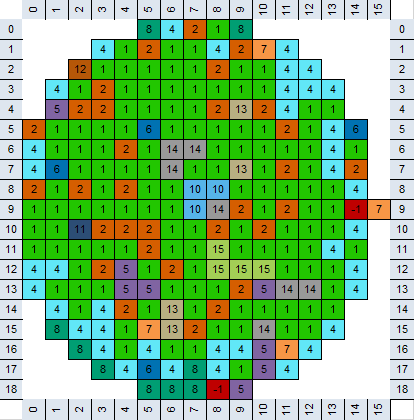
\includegraphics[width=0.5\textwidth]{showNum.png}
	\caption{Bin numbers visible with showNum}
	\label{fig:showNum}
\end{figure}

\section{\bf Histograms}
\subsection{\bf -h or \texttt{-{}-}genHistograms}
\subsubsection{\bf -B or \texttt{-{}-}manualBins}
By default, the number of bins for each histogram is automatically calculated using a modified version of Scott's normal reference rule. Manually setting this value will apply the same number of bins across all histograms, except for the ones that have only one bin.
\subsubsection{\bf -C or \texttt{-{}-}cutOutlier}
This defines how much of the outlier data should be excluded from histogram view, in terms of standard deviation. By default the cutoff is 1.5, which means that any data outside the range of mean$\pm$1.5$\sigma$ is excluded. To disable cutoff altogether, set this option to 0.

\end{document}
